\section*{ Arquitectura}\label{sec:arq}

A biblioteca vai seguir um modelo de programa��o modular em que cada m�dulo ir� ter uma responsabilidade diferente.
Existir� um modulo comum onde estar�o implementados os algoritmos e onde
estar� definida uma interface que estandardize as interfaces disponibilizadas pelas diversas plataformas. Esta interface estandardizada e comum
a todos os m�dulos ter� o objectivo de permitir a implementa��o dos algoritmos de forma independente da plataforma.
Para cada plataforma estudada (Apache Hama, Apache Giraph e GPS) ser� efectuado um m�dulo cuja fun��o � a de mapear a interface da respectiva plataforma para a interface
estandardizada.

\begin{figure}[h]
  \centering
  \caption{Arquitectura modular da biblioteca.}
  \scalebox{0.5}{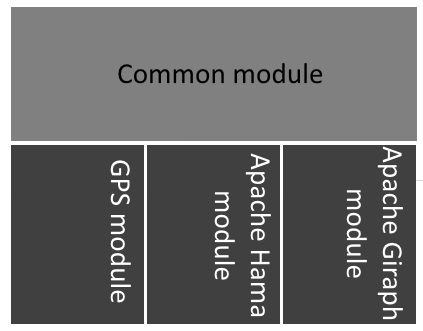
\includegraphics{arq_idea.png}}%\\
  \label{arq_idea}
\end{figure}
